\section{Module 1}

\subsection{Red Box!}
\begin{itemize}
    \item User mode and kernel mode are important concepts!
    (Section 1.4.2 in Operating System Concepts)
    \item Handling a system call. (Covered in section 2.3.2 in Operating System Concepts)
    \item OS structures, important to understand the different structures (monolithic, layered, microkernels, modules and hybrid systems) and their trade-offs. Covered in section 2.8 in Operating System Concepts.
\end{itemize}

\subsection{User and Kernel mode}

\paragraph{What are User Mode and Kernel Mode?}
User mode and kernel mode are two distinct execution modes in a computer system that separate the level of privilege and access to system resources. This separation ensures system stability and security.

\begin{itemize}
    \item \textbf{User Mode:}
    \begin{itemize}
        \item The mode in which user applications run.
        \item Access to system resources and hardware is restricted.
        \item System calls must be used to request services from the operating system.
    \end{itemize}
    
    \item \textbf{Kernel Mode:}
    \begin{itemize}
        \item The mode in which the operating system runs.
        \item Full access to all system resources, including hardware and memory.
        \item Executes critical tasks like process management, memory management, and device handling.
    \end{itemize}
\end{itemize}

\paragraph{Why are User Mode and Kernel Mode Important?}
\begin{itemize}
    \item They ensure system stability by preventing user applications from directly accessing or modifying critical system resources.
    \item They enhance security by isolating user applications from the operating system kernel.
    \item They enable efficient multitasking and resource management by allowing the operating system to control access to hardware and shared resources.
\end{itemize}





\subsection{System Call}


\paragraph{What is a System Call?}
A system call is a mechanism used by user-level applications to request services from the operating system's kernel. These services include operations like file manipulation, process management, and memory allocation.

\paragraph{Steps in Handling a System Call:}
\begin{enumerate}
    \item \textbf{Triggering the System Call:}
    \begin{itemize}
        \item The user application invokes a system call, typically through a library function.
        \item A special CPU instruction, such as \texttt{INT} (Interrupt) or \texttt{SYSENTER}, switches the execution mode from user mode to kernel mode.
    \end{itemize}
    
    \item \textbf{Identifying the System Call:}
    \begin{itemize}
        \item The system call number is passed to the kernel, usually via a specific register or stack.
        \item The kernel uses this number to determine the requested service.
    \end{itemize}
    
    \item \textbf{Processing the Request:}
    \begin{itemize}
        \item The kernel executes the corresponding system call handler.
        \item This may involve interacting with hardware, managing resources, or performing calculations.
    \end{itemize}
    
    \item \textbf{Returning to User Mode:}
    \begin{itemize}
        \item The kernel completes the system call and prepares the return value or status.
        \item The CPU switches back to user mode, and the control returns to the user application.
    \end{itemize}
\end{enumerate}

\paragraph{Example:}
For a \texttt{read()} system call:
\begin{itemize}
    \item The application calls \texttt{read()}, specifying the file descriptor, buffer, and size.
    \item The kernel checks permissions, retrieves the data from the file, and writes it to the buffer.
    \item The system call returns the number of bytes read or an error code.
\end{itemize}


\begin{figure}[H]
    \centering
    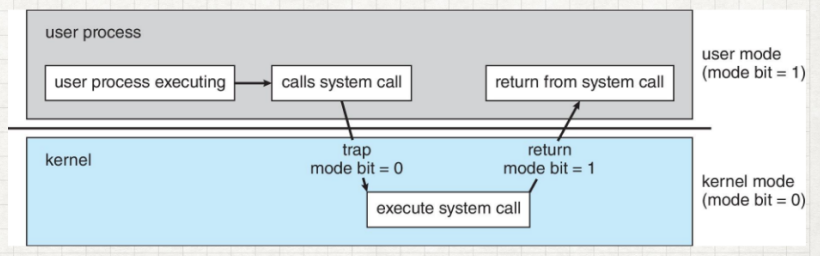
\includegraphics[width=0.8\textwidth]{syscall.png}
    \caption{Diagram of a system call.}
    \label{fig:syscall}
\end{figure}


\subsection{OS Structures}

\paragraph{Monolithic Structure}
\begin{itemize}
    \item \textbf{Description:} All OS components are contained in a single, large kernel.
    \item \textbf{Advantages:}
    \begin{itemize}
        \item High performance due to minimal communication overhead.
        \item Simple to implement and efficient for tightly coupled systems.
    \end{itemize}
    \item \textbf{Disadvantages:}
    \begin{itemize}
        \item Difficult to maintain and debug due to lack of modularity.
        \item A single failure can compromise the entire system.
    \end{itemize}
\end{itemize}

\paragraph{Layered Structure}
\begin{itemize}
    \item \textbf{Description:} OS is divided into layers, each built on top of the other, with clear interfaces.
    \item \textbf{Advantages:}
    \begin{itemize}
        \item Easier to maintain and extend due to modular design.
        \item Improves security and stability by isolating functionalities.
    \end{itemize}
    \item \textbf{Disadvantages:}
    \begin{itemize}
        \item Overhead from inter-layer communication.
        \item Can be less efficient due to strict layering.
    \end{itemize}
\end{itemize}

\paragraph{Microkernels}
\begin{itemize}
    \item \textbf{Description:} Minimal kernel providing core functions like communication and basic scheduling, with other services running in user space.
    \item \textbf{Advantages:}
    \begin{itemize}
        \item Highly modular and easier to extend or modify.
        \item Improved security and reliability since most services run in user mode.
    \end{itemize}
    \item \textbf{Disadvantages:}
    \begin{itemize}
        \item Higher communication overhead between user space and kernel.
        \item Slower performance compared to monolithic kernels.
    \end{itemize}
\end{itemize}

\paragraph{Modules}
\begin{itemize}
    \item \textbf{Description:} The OS kernel is extensible via loadable modules, which can be dynamically added or removed. This type of design is common in modern implementations
    of UNIX , such as Linux, macOS, and Solaris, as well as Windows. 
    \item \textbf{Advantages:}
    \begin{itemize}
        \item Combines the efficiency of monolithic kernels with the flexibility of modularity.
        \item Reduces the kernel size by loading only necessary modules.
    \end{itemize}
    \item \textbf{Disadvantages:}
    \begin{itemize}
        \item Compatibility issues may arise between modules.
        \item Bugs in modules can still compromise the kernel.
    \end{itemize}
\end{itemize}

\paragraph{Hybrid Systems}
\begin{itemize}
    \item \textbf{Description:} A combination of microkernel and monolithic design, incorporating the benefits of both.
    \item \textbf{Advantages:}
    \begin{itemize}
        \item Balances performance and modularity.
        \item Adaptable to various system requirements.
    \end{itemize}
    \item \textbf{Disadvantages:}
    \begin{itemize}
        \item Increased complexity in design and implementation.
        \item May not fully exploit the advantages of either microkernels or monolithic kernels.
    \end{itemize}
\end{itemize}